\documentclass[a4paper,12pt]{jsarticle}
\bibliographystyle{junsrt}
\usepackage{ascmac}
\usepackage{empheq}
\usepackage{amsmath,amssymb}
\usepackage{bm}
\usepackage[dvipdfmx]{graphicx,color}
\usepackage[top=30truemm,bottom=30truemm,left=40truemm,right=40truemm]{geometry}
\usepackage{here}
\usepackage{comment}
\title{レーザー歪み計を用いた基線長安定化制御の提案}
\author{三代浩世希}
\begin{document}
\setcounter{tocdepth}{3}
\maketitle
\abstract{}
\tableofcontents

\section{GIFをつかった能動防振}
\subsection{能動防振}


能動防振システムの性能は以下の3つで評価できる
\begin{enumerate}
\item \textbf{外乱抑制性能} ステージへの地面振動の流入をどれぐら抑えられるか 
\item \textbf{即応性能} RMSをどれぐらい小さく抑えられるか
\item \textbf{目標値追従性能} 干渉計からの制御信号にどれぐらい追従させられるか
\end{enumerate}

ダンピング制御のようなDCにFeedBackゲインをもつ必要がない制御の場合、FeedBack制御だけで外乱抑制と即応性を向上するように最適なパラメータを設計できるが、目標値への追従性能は返って悪くなる。防振装置はテストマスのダンピング制御だけではなく位置制御も必要であるので、2自由度制御\cite{taguchi2000two}とよばれる、目標追従性能も同時に向上させることのできる制御をもちいなければならない。

%% 重力波望遠鏡の鏡は地面振動雑音を低減するように振り子で吊られている。これにより共振周波数以上の帯域では鏡は慣性系に対して静止するようになる。そのため、より低周波で感度をもつために、より低い共振周波数の振り子を多段で組み合わせる工夫がなされている。しかしデザイン感度を満たす振り子であっても、干渉計が限られたダイナミックレンジの中で動作できるようRMSを小さくすることができなければ、望遠鏡として安定して動かすことはできない。

%% 基線長変動のRMSは感度帯域より低周波の地面振動が大きく寄与している(図1)。0.2Hzのピークは脈動と呼ばれ、波浪が海底面を叩くことが原因である。脈動の振幅は波高と相関があり、その周期は浅瀬の深さに依存していることが知られている\cite{kedar2008origin}。更に低周波の$10^{-5}\, \mathrm{Hz}$のピークは地球潮汐と呼ばれ、地球と月の潮汐力によって引き起こされる。



\subsection{LIGOの能動防振}
\begin{figure}[H]
  \begin{center}
    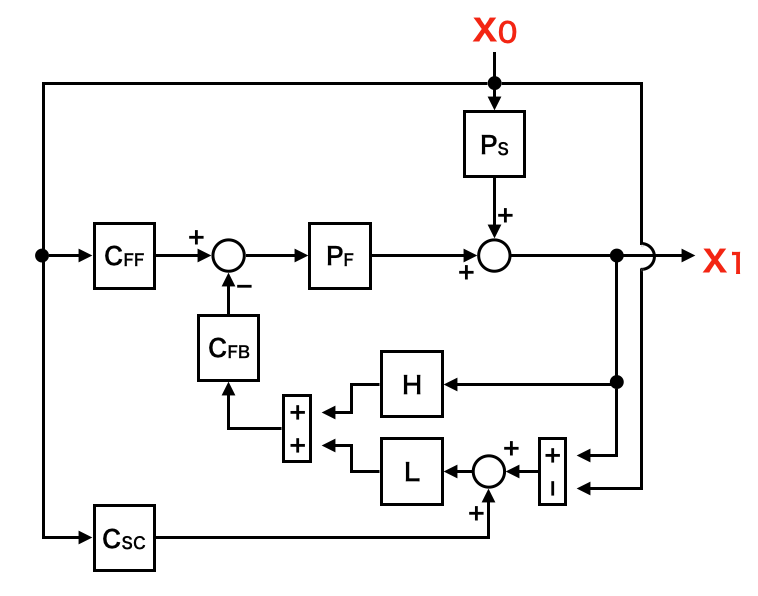
\includegraphics[width=11.5cm]{./img_2dof_pi.png}
  \end{center}
  \caption{Preisolatorで用いている能動防振のブロック図。ここで、$P_{\mathrm{s}}$は地面振動の変位$x_0$からステージの変位$x_1$への伝達関数である。$C_{\mathrm{fb}},\,C_{\mathrm{ff}},\,C_{\mathrm{sc}}$はそれぞれ feedback、feedforward、sensor correctionの制御フィルターである。さらに$H,\,L$はsuper sensor のための相補フィルターであり、それぞれ慣性センサーのためのハイパスフィルターと変位センサーのためのローパスフィルターである。また$N_{ff},\,N_{sc},\,N_{H},\,N_{L}$はそれぞれのセンサーのノイズとなっている。そして$G$はループゲインをあらわしており$G=C_{\mathrm{fb}}P_{\mathrm{f}}$という関係であり、このときの$P_{\mathrm{f}}$はステージのアクチュエータからステージの変位への伝達関数である。}\label{img:img_2dof_pi}
\end{figure}

Preisolatorの目的はステージの変位を慣性系に対して静止させることであるため、FeedBackで用いるセンサーには慣性センサーを用いなければならない。しかし一般的に慣性センサーは低周波でノイズが大きい。そのためDCでループゲインをもたせることができず、ダンピングをするためにしか使うことができない(Inertial Damping)。

一方で共振器長制御のためにステージの位置制御をしなければならないため、妥協案として低周波ではローカルな変位センサーをつかって低周波では地面にロックしている。これは比較的小さいスケールの腕共振器であれば、ITMとETMは同相で地面に揺らされて、低周波地面振動は同相雑音として除去されるので問題とならない。しかしkmスケールの腕共振器では、RMSの大きな脈動の帯域では、逆相成分である基線長伸縮は同相成分とくらべて1/4程度にしか低減できない。このような問題を解決するためにLIGOではsensor correction と呼ばれるfeed forward 制御を用いて脈動の補償をしている\cite{matichard2015seismic}。

図\ref{img:img_2dof_pi}に示したLIGOの能動防振のブロック図において、ステージの変位$x_1$を地面振動$x_0$と目標値$r$で表すと式(\ref{eq:eq04})の通りである。
\begin{eqnarray} \label{eq:eq04}
  x_1 &=& \frac{1}{1+G}\Biggl[(P_{\mathrm{s}}+P_{\mathrm{f}}C_{\mathrm{ff}})x_0\Biggl]
  + \frac{G}{1+G}\Biggl[L(1+C_{\mathrm{sc}})x_0\Biggl]
\end{eqnarray}
ここで外乱抑制を高めるためにゲインを十分におおきくすると式(\ref{eq:eq06})になる。式(\ref{eq:eq07})のとおり feed back のみの場合はステージの変位$x_1$はローパスフィルター$L$に沿って地面振動$x_0$を流入させるが、sensor correction を加えて適当な$C_{\mathrm{sc}}$と目標値$r$を選べばゼロにすることができる。
\begin{eqnarray}\label{eq:eq06}
  \lim_{G \to \infty} x_{1} &=& L(x_{0}+C_{\mathrm{sc}}r) \\
  &=&
  \begin{cases}\label{eq:eq07}
    \; Lx_{0} & \text{($C_{\mathrm{sc}}=0$)}\\
    \; 0 & \text{($-C_{\mathrm{sc}}r=x_0$)} 
  \end{cases}  
\end{eqnarray}
LIGOの場合、目標値$r$に、地面に設置した地震計の信号を入れている。

さらに高周波帯域のステージの要求値を満たすために、sensor correction とは別の feed forward のパスを用意している。式(\ref{eq:eq08})にゲインを小さくした場合のステージの変位$x_1$を示す。このとき、式(\ref{eq:eq09})のとおり、feed forwardがない場合は地面振動でステージの変位は制限されるが、sensor correction と同様に、適当な$C_{\mathrm{ff}}$と$r$を選べば、地面振動からの寄与を減らすことができる。
\begin{eqnarray}\label{eq:eq08}
  \lim_{G \to 0} x_{1} &=& P_{\mathrm{s}}x_0 + P_{\mathrm{f}}C_{\mathrm{ff}}r \\
  &=& 
  \begin{cases}\label{eq:eq09}
    \; P_{\mathrm{s}}x_{0} & \text{($C_{\mathrm{ff}}=0$)}\\
    \; 0 & \text{($-P_{\mathrm{f}}C_{\mathrm{ff}}r=P_{\mathrm{s}}x_0$)} 
  \end{cases}  
\end{eqnarray}
実際の目標値には、sensor correction と同様に、地震計出力を入れている。2つの feed forward に用いる地震計には

\subsection{KAGRAの能動防振}




\begin{figure}[H]
  \begin{center}
    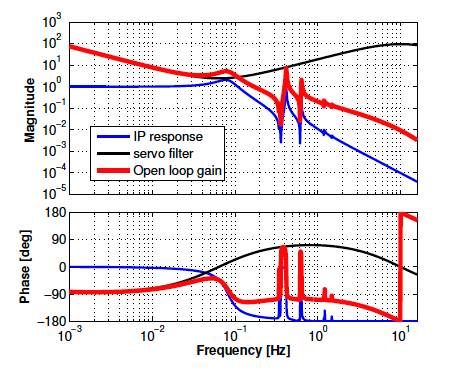
\includegraphics[width=11.5cm]{./img_ip_servo.png}
  \end{center}
  \caption{}\label{img:img_ip_servo}
\end{figure}



%% 地面振動$x_0$とステージの変位$x_1$に注目すると、地面振動からステージへの伝達関数は、
%% \begin{eqnarray}\label{eq:eq05}
%%   \frac{x_1}{x_0} = \frac{1}{1+G}P_{S}\Biggl[1-\frac{P_{f}}{P_{S}}C_{FF}\Biggl] + \frac{G}{1+G}L(1-C_{SC}) 
%% \end{eqnarray}
%% になる。ここでループゲインを十分大きくすると、式(\ref{eq:eq05})の地面振動からの直接の寄与(第1項)は十分に小さくできるが、変位センサーからの流入(第2項)はのこる。つまり、
%% \begin{eqnarray}\label{eq:eq06}
%%   \lim_{G \to \infty} \biggl(\frac{x_1}{x_0}\biggl) = L(1-C_{SC})
%% \end{eqnarray}
%% となる。先述した変位センサをFeedback制御に使う問題は、$C_{SC}=C_{FF}=0$とすれば$x_1/x_0=L$と表現し直すことができる。つまりカットオフ周波数以下ではステージと地面は一緒になって動くことを意味する。したがってそうならないように、$L$の寄与を小さくしたい。まず$C_{FF}=0$ の状態で考えると、sensor correction のフィルター$C_{SC}$を全域で1にできれば可能である。しかし実際には sensor correction で使用する慣性センサーもまた低周波で地面振動よりもノイズが大きくなるので、ノイズを流入させないように十分高次なハイパスフィルターを設計する必要がある。






\appendix
\section{2自由度制御}

\begin{figure}[H]
  \begin{center}
    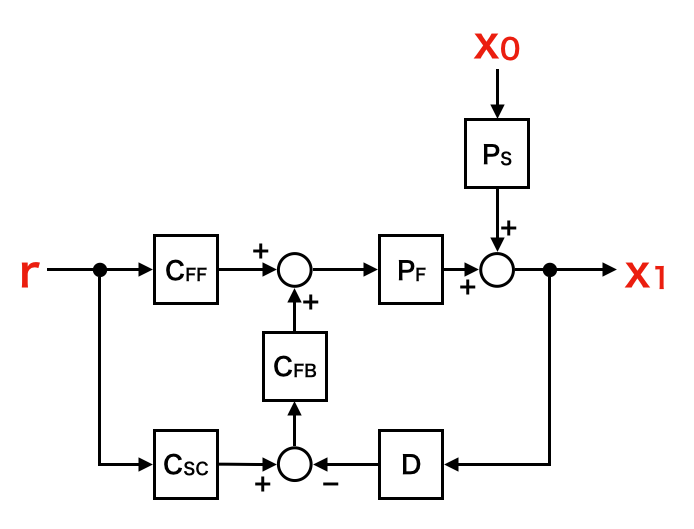
\includegraphics[width=11.5cm]{./img_2dof.png}
  \end{center}
  \caption{}\label{img:img_2dof}
\end{figure}

能動防振でつかわれている2自由度制御を説明するよりも先に、2自由度制御のひな形を用いて、2自由度制御の利点である、外乱抑制性能と目標追従性能の両方を向上できることを示しておかなければならない。まずステージの変位$x_1$を目標値$r$と外乱$x_0$で表すと式(\ref{eq:eqA01})のとおりになる。
\begin{eqnarray} \label{eq:eqA01}
  x_1 &=& \frac{1}{1+G}\Biggl[P_{\mathrm{s}}x_0 + P_{\mathrm{f}}C_{\mathrm{ff}}r\Biggl] + \frac{G}{1+G}\Biggl[\frac{C_{\mathrm{sc}}}{D}\Biggl]r
\end{eqnarray}
もし$C_{\mathrm{ff}}=1$かつ$C_{\mathrm{sc}}=0$であれば一般的なFeedBack制御になるが、2自由度制御では式(\ref{eq:eqA01})の第2項が加わるおかげで外乱抑制と目的値追従を両方とも良くすることができる。それはつまり外乱抑制をよくするためにGを大きくとると、
\begin{eqnarray} \label{eq:eqA02}
  \lim_{G \to \infty} x_1 = \frac{C_{SC}}{D}r
\end{eqnarray}
となり、適当な$C_{\mathrm{sc}}$を選べば、$x_{1}=r$となって、制御後の値$x_{1}$を目標値$r$に一致させることができるためである。

\section{式置き場}

\begin{eqnarray}
  d_1 &=& \frac{1}{1+G}P_{S}d_0 \\
  &+& \frac{G}{1+G}\Biggl[L(1-C_{SC})-\frac{C_{FF}+C_{GIF}}{C_{FB}}\Biggl]d_0 \nonumber \\
  &-& \frac{G}{1+G}\Biggl[HN_{H} + LN_{SC} + LN_{L} + \frac{C_{FF}}{C_{FB}}N_{FF} + \frac{C_{GIF}}{C_{FB}}N_{GIF} \Biggl] \nonumber
\end{eqnarray}

\begin{eqnarray}
  \lim_{G \to \infty} \langle|d_1|^2\rangle =
  \biggl\langle\biggl|[L(1-C_{SC})-\frac{C_{FF}+C_{GIF}}{C_{FB}}]d_0\biggl|^2\biggl\rangle + \langle|N_{\mathrm{all}}|^2 \rangle \\
N_{\mathrm{all}} \equiv HN_{H} + LN_{SC} + LN_{L} + \frac{C_{FF}}{C_{FB}}N_{FF} + \frac{C_{GIF}}{C_{FB}}N_{GIF} \nonumber
\end{eqnarray}
%
%
\begin{eqnarray}
  x_1 &=& \frac{1}{1+G}\Biggl[(P_{\mathrm{s}}+P_{\mathrm{f}}C_{\mathrm{ff}})x_0\Biggl]
  + \frac{G}{1+G}\Biggl[L(1+C_{\mathrm{sc}})x_0 + r\Biggl]
\end{eqnarray}


\bibliography{./reference}

\end{document}
